% updated April 2002 by Antje Endemann
% Based on CVPR 07 and LNCS, with modifications by DAF, AZ and elle, 2008 and AA, 2010, and CC, 2011; TT, 2014; AAS, 2016; AAS, 2020

\documentclass[runningheads]{llncs}
\usepackage{graphicx}
\usepackage{comment}
\usepackage{amsmath,amssymb} % define this before the line numbering.
\usepackage{color}

% INITIAL SUBMISSION - The following two lines are NOT commented
% CAMERA READY - Comment OUT the following two lines
\usepackage{ruler}
\usepackage[width=122mm,left=12mm,paperwidth=146mm,height=193mm,top=12mm,paperheight=217mm]{geometry}

\usepackage{amsmath}
\usepackage{amssymb}
\usepackage{mathrsfs}
\usepackage{amssymb}
\usepackage{multirow}
\usepackage{subfigure}
\usepackage{booktabs}
\usepackage{floatrow}
\graphicspath{{pic/}}

% Include other packages here, before hyperref.

% If you comment hyperref and then uncomment it, you should delete
% egpaper.aux before re-running latex.  (Or just hit 'q' on the first latex
% run, let it finish, and you should be clear).
\usepackage[pagebackref=true,breaklinks=true,letterpaper=true,colorlinks,bookmarks=false]{hyperref}


\begin{document}
% \renewcommand\thelinenumber{\color[rgb]{0.2,0.5,0.8}\normalfont\sffamily\scriptsize\arabic{linenumber}\color[rgb]{0,0,0}}
% \renewcommand\makeLineNumber {\hss\thelinenumber\ \hspace{6mm} \rlap{\hskip\textwidth\ \hspace{6.5mm}\thelinenumber}}
% \linenumbers
\pagestyle{headings}
\mainmatter
\def\ECCVSubNumber{242}  % Insert your submission number here

\title{Exploring global point context for 3D detection} % Replace with your title

% INITIAL SUBMISSION 
%\begin{comment}
\titlerunning{ECCV-20 submission ID \ECCVSubNumber} 
\authorrunning{ECCV-20 submission ID \ECCVSubNumber} 
\author{Anonymous ECCV submission}
\institute{Paper ID \ECCVSubNumber}
%\end{comment}
%******************

% CAMERA READY SUBMISSION
\begin{comment}
\titlerunning{Abbreviated paper title}
% If the paper title is too long for the running head, you can set
% an abbreviated paper title here
%
\author{Xu Liu\inst{1}\orcidID{0000-1111-2222-3333} \and
Jian Wang\inst{2,3}\orcidID{1111-2222-3333-4444} \and
Boxin Shi\inst{2,3}\orcidID{1111-2222-3333-4444} \and
Xiaodong He\inst{1}\orcidID{2222--3333-4444-5555}}
%
\authorrunning{F. Author et al.}
% First names are abbreviated in the running head.
% If there are more than two authors, 'et al.' is used.
%
\institute{Princeton University, Princeton NJ 08544, USA \and
Springer Heidelberg, Tiergartenstr. 17, 69121 Heidelberg, Germany
\email{lncs@springer.com}\\
\url{http://www.springer.com/gp/computer-science/lncs} \and
ABC Institute, Rupert-Karls-University Heidelberg, Heidelberg, Germany\\
\email{\{abc,lncs\}@uni-heidelberg.de}}
\end{comment}
%******************
\maketitle

\begin{abstract}
%The abstract should summarize the contents of the paper. LNCS guidelines
%indicate it should be at least 70 and at most 150 words. It should be set in 9-point
%font size and should be inset 1.0~cm from the right and left margins.
\dots
\keywords{3D Point Cloud, Object Detection, Contextual feature}
\end{abstract}


\section{Introduction}
The challenging task of object detection with 3D point cloud plays a key role for Autonomous Driving and Robotics. Previous methods  like \cite{voxelnet} leverage this problem by partitioning the 3D space into regular sized voxels or transforming into the BEV(Bird Eye View) \cite{pixor} and then apply the conventional CNN methods.
However, the initial quantization process of these methods will inevitably introduces the quantization error and this may inhibit the performance of the algorithm.

Recently, the PointNet/PointNet++ \cite{pointnet,pointnet++} has shed lights  on modeling the 3D point clouds directly from the raw-input, thus the quantization error can be avoided. The PointNet++ utilized a series  of Set Abstraction or SA operators to enlarge the receptive field gradually and obtain global information. 

 The global contextual clues in the complex indoor environment is beneficial for scene understanding. For instance,  the table in the meeting room should be surrounded by the chairs; this  global contextual information and the inherent relationship can make it easy  to narrow down the type of the object among the long category list. The ability of PointNet++ \cite{pointnet++} to encode the context information has enabled  VoteNet \cite{VoteNet} and PointRCNN \cite{PointRCNN} to achieve  state-of-the-art performance on prevailing benchmarks like  \cite{SUN_RGBD,SCannet} and \cite{Kitti}. However, it is not instinctive enough to obtain the global contextual information with this approach. Since the global information may still be unreachable beyond the range of the largest receptive field. %not intuitive enough 

Recently, there have been new methods to acquire global context, such as global spatial-wise  attention  Global context  by \cite{LG-PointNet++}.

However, the computational cost of spatial is heavy, it requires the intensive computing of feature among the point pairs, as shown in Figure \ref{fig:Flyer}. (a)

To better understand the  the problem,  we make the following analysis. Let high dimensional feature space represented by$\Omega$, which can be expressed by $\Omega= S \times C$. And $S$ stands for the spatial domain and $C$ stands for channel domain. $S$ is just a partial observation of $\Omega$. The separation of spatial context in $S$ with the channel dimension has cut off the relations among the points, as a result,  redundancy of the data is increased. And the computation cost has increased correspondinly.

 To avoid the issue mentioned above, the global context should be acquired directly from the high dimensional feature space $\Omega$ and the statistical method should be leveraged to for this problem. In the era of statistical learning, the global context of the image/language are obtained intuitively by encoding the features with the dictionary, or the set of  codewords in the feature space. The features are encoded with the dictionary by such methods like BoW \cite{BoW1,BoW2,BoW3,BoW4}, and residual encoding methods like VLAD\cite{VLAD}, and Fisher Vector \cite{FisherVector1,FisherVector2}.  Inspired by such theories, Zhang et al proposed an end-to-end,  differentiable encoding layer \cite{DeepTEN} that encompass the function of dictionary learning and  residual encoding. This design has been proved successful for texture encoding \cite{DeepTEN} and other 2D tasks  \cite{encnet,pascal,ImageNet}, thus  motivating us to leverage this design in 2D tasks to exploit the global contextual information in the 3D point clouds.
 
\begin{figure}[t]
\label{fig:Flyer}
			\begin{minipage}{1\textwidth}
				\centering
				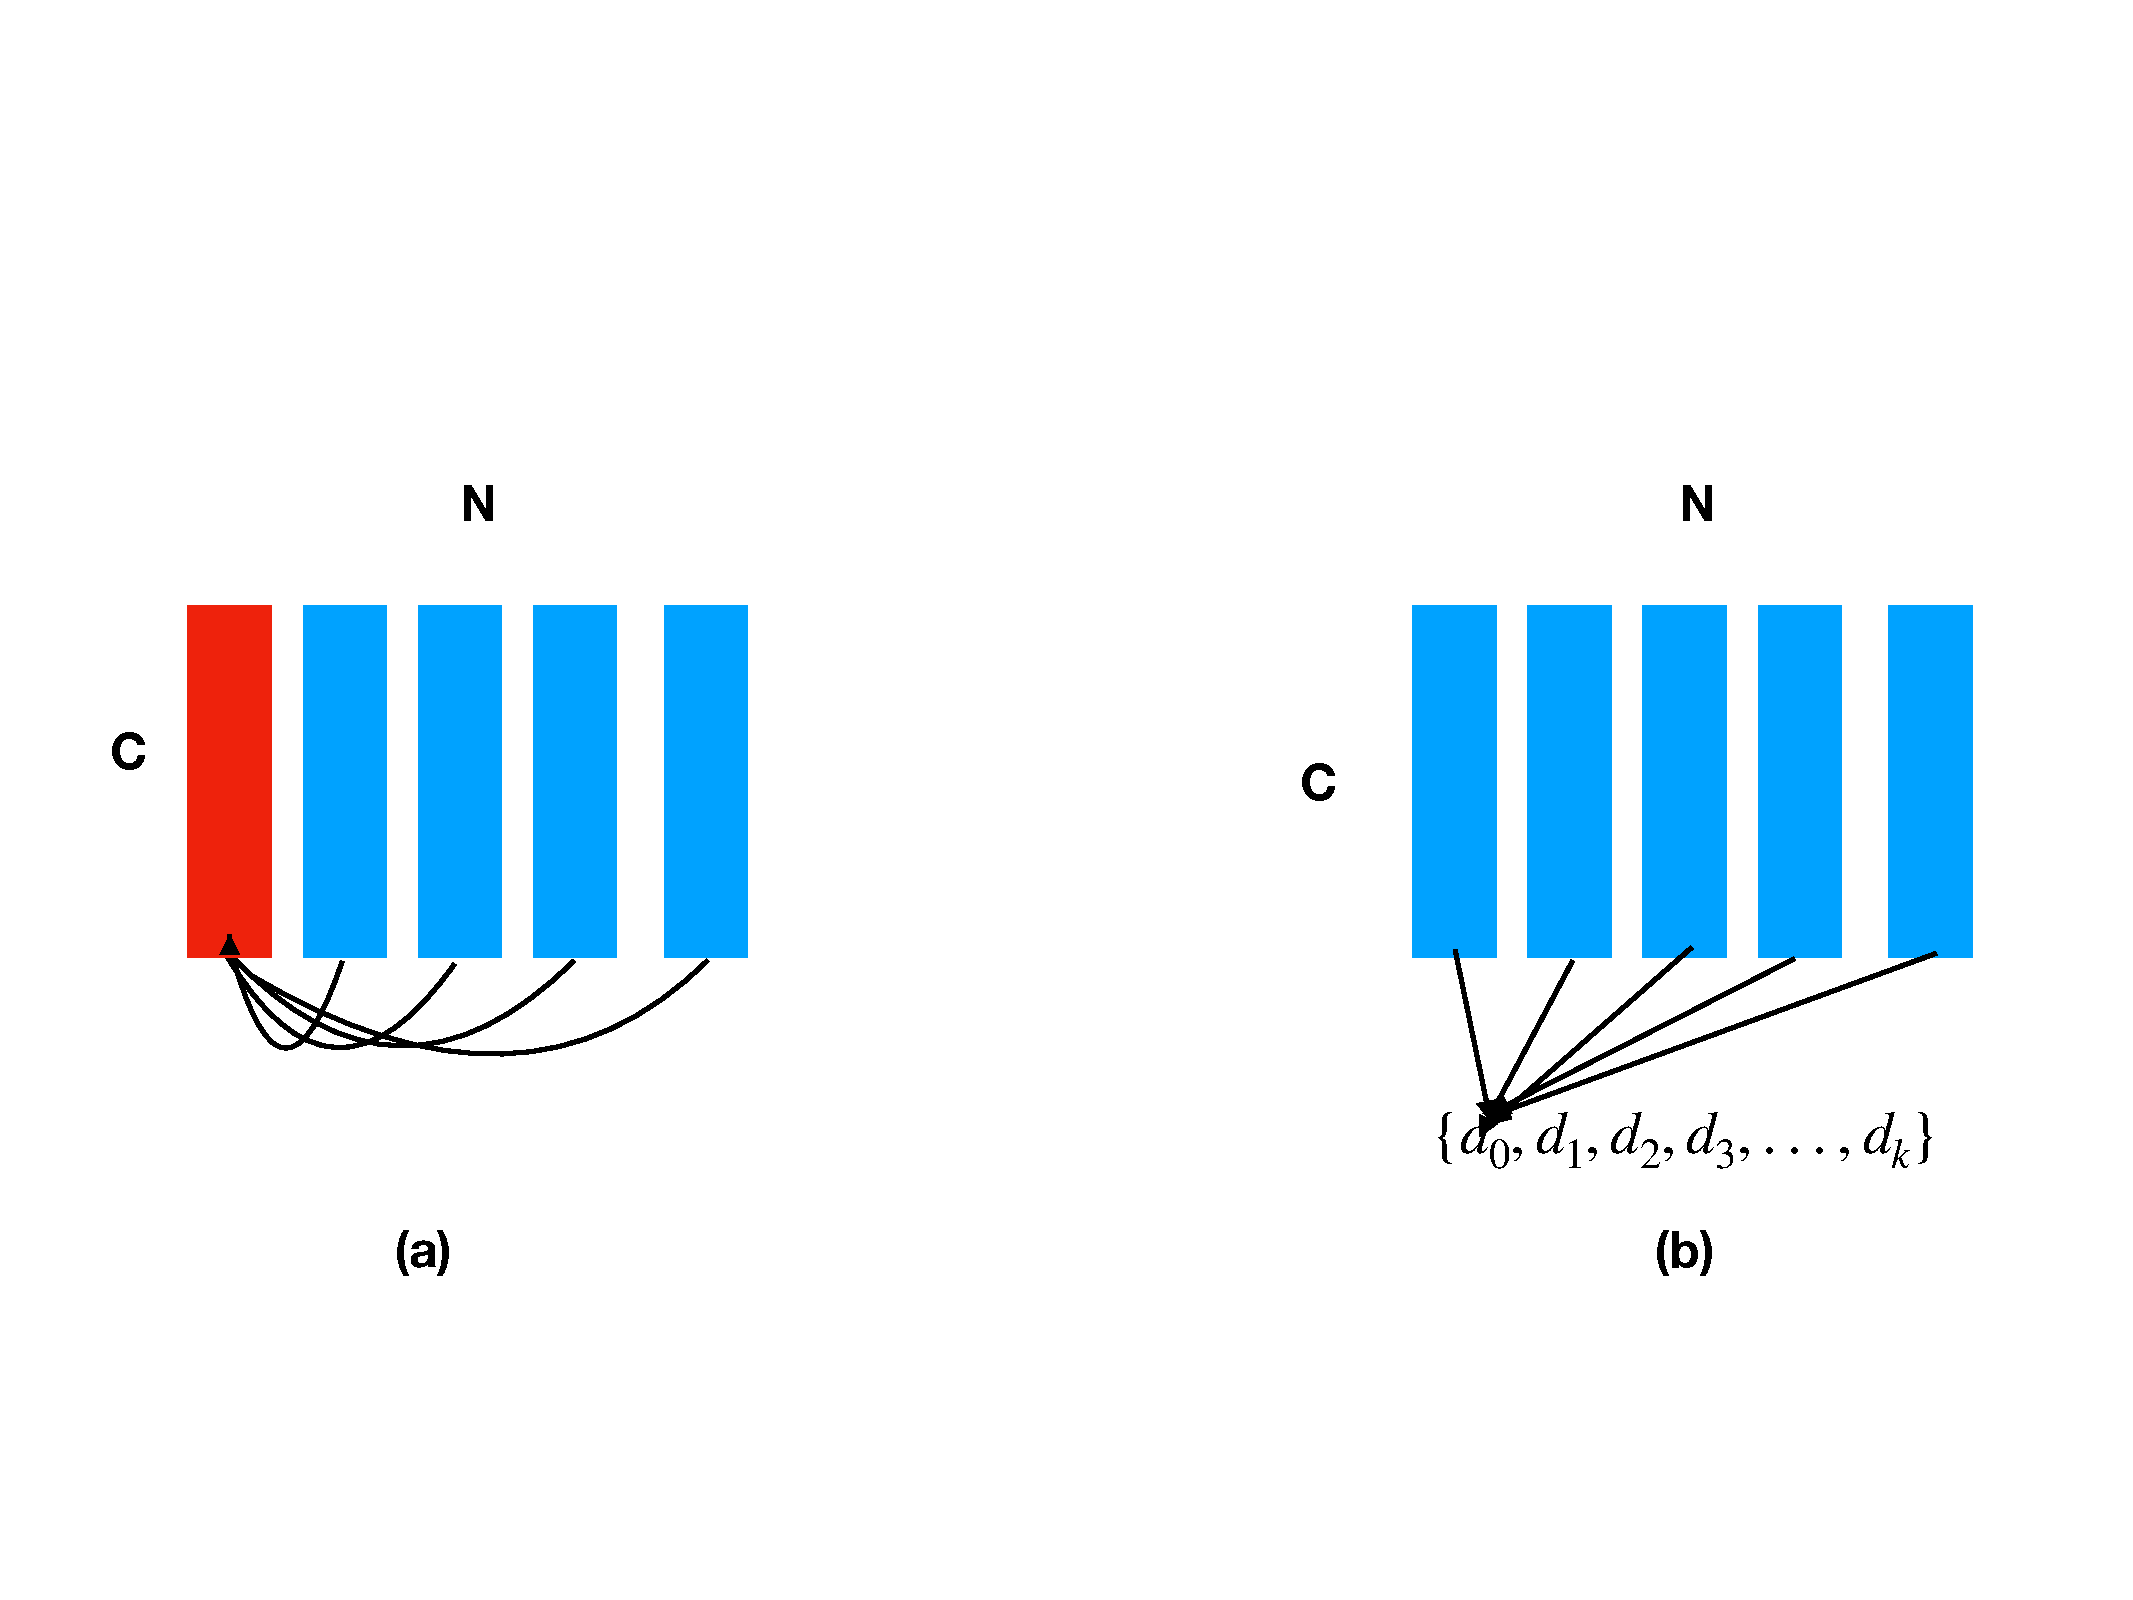
\includegraphics[width=1.0\linewidth]{eccv2020kit/Figure/Flyer.pdf}
			\end{minipage}
    \caption{To acquire global context, the method of global spatial attention in Figure \ref{fig:Flyer} (a) intensively aggreagate the features between N point pairs. We propose an efficient  way in Figure \ref{fig:flyer} (b) to represent  global context  with  a few K independent code-words, which is more efficient..  }%
\label{fig:flyer}
    
\end{figure}
 
In this work, we  propose the \emph{Point Contextual Encoding Module} to exploit the global context efficiently  with only a few code words in the high dimensional feature space. which is illustrated in Figure \ref{fig:Flyer} (b). This global context will then be Incorporated with the point features for better representations.% Compared with the method of global spatial context, our method is computation economical because the features will be encoded by only a few numbers of the codeword. Compared with channel context, our method is able to deal with the geometric scenes of the point cloud. 
 

 
The contributions of our paper are in the following aspects:
\begin{itemize}
    \item %We are the first attempting to capture the global context of point cloud for 3D detection. To achieve this goal,
    We proposed the \emph{Point Contextual Encoding Module} by incorporating the Encoding Layer to capture global information of the point sets, %then use this information
    this global contextual information is then used to modulate the channel-wise embedding of the Point Set features. So that it can highlight or de-emphasize the featuremap  according to the global contextual priors.
    
    \item
    Our method is able to obtain the global context directly from high dimensional feature space. Compared with the partial spatial and channel context methods, our method keeps the balance between computation cost and representation abilities.
    
    \item  By utilizing the  \emph{Point Contextual Encoding Module}  as the building block and following the design of PointNet++ , the feature representation has been improved by the global contextual information  \emph{Point Contextual Encoding Module}. This has been verified on the challenging 3D detection tasks.
 
    
\end{itemize}

\section{Related Works}
\label{related_works}

\noindent{\textbf{PointNet++ Architecture}}

In recent years,  methods \cite{pointcnn,sawnet,ASIS,kpconv,shape_matching,shapecontextnet} have been proposed to design end-to-end models for point cloud. Pioneering work of PointNet \cite{pointnet}  model the point cloud directly from the raw input data. Then PointNet++ \cite{pointnet++}  introduces  Set Abstraction (SA) - Feature Propagation (FP) paired encoder-decoder  structure: The SA operators  will enlarge the receptive field and reduce the point number sequentially in the phase of encoder . Then in the deccoder phase, the FP operators are utilized to recover the point number and fuse the skip-connected features of different layers. This structure lacks the ability to acquire global context effectively.

\noindent{\textbf{Context in 3D point clouds}}

To explore the relationships between the  points, Zhao et al. proposed the \cite{pointweb} to exploit the local context among the neighbours. This method has its limitation to obtain the global context of the entire scene.

\cite{ppfnet} and  \cite{LG-PointNet++} is pioneering in obtaining global context for 
point cloud segmentation.  But the global feature is computed by scanning each pair or local patches intensively, which is computational expensive for the dense-clustered indoor scenes.


In comparison with our method,  the global context is computed by encoding with only a few numbers of code words in the dictionary of the encoding layer, which is computational economical.



\noindent{\textbf{PointNet++ based detectors}}

The current detectors  \cite{VoteNet,PointRCNN,STD} typically adopt PointNet++  mentioned above as the backbone to model the raw input of point clouds. Among these detectors, PointRCNN \cite{PointRCNN} and STD \cite{STD} can be classified into the category of \emph{two-stage} detector, %of their bottom-up proposal generation network in the first stage. 
while VoteNet \cite{VoteNet} is a \emph{one stage} single shot 3D detection network. 


\noindent{\textbf{Context in 2D}} 
%\subsection{Context in 2D}

Methods of \cite{Deeplabv1,Deeplabv3,Deeplabv3+,DenseASPP,largekernel,SENet,encnet} in 2D introduce efficient ways of multi-scale contextual feature aggregation and some of the methods has been leveraged for  3D problems.


\begin{figure}[t]
			\begin{minipage}{1\textwidth}
				\centering				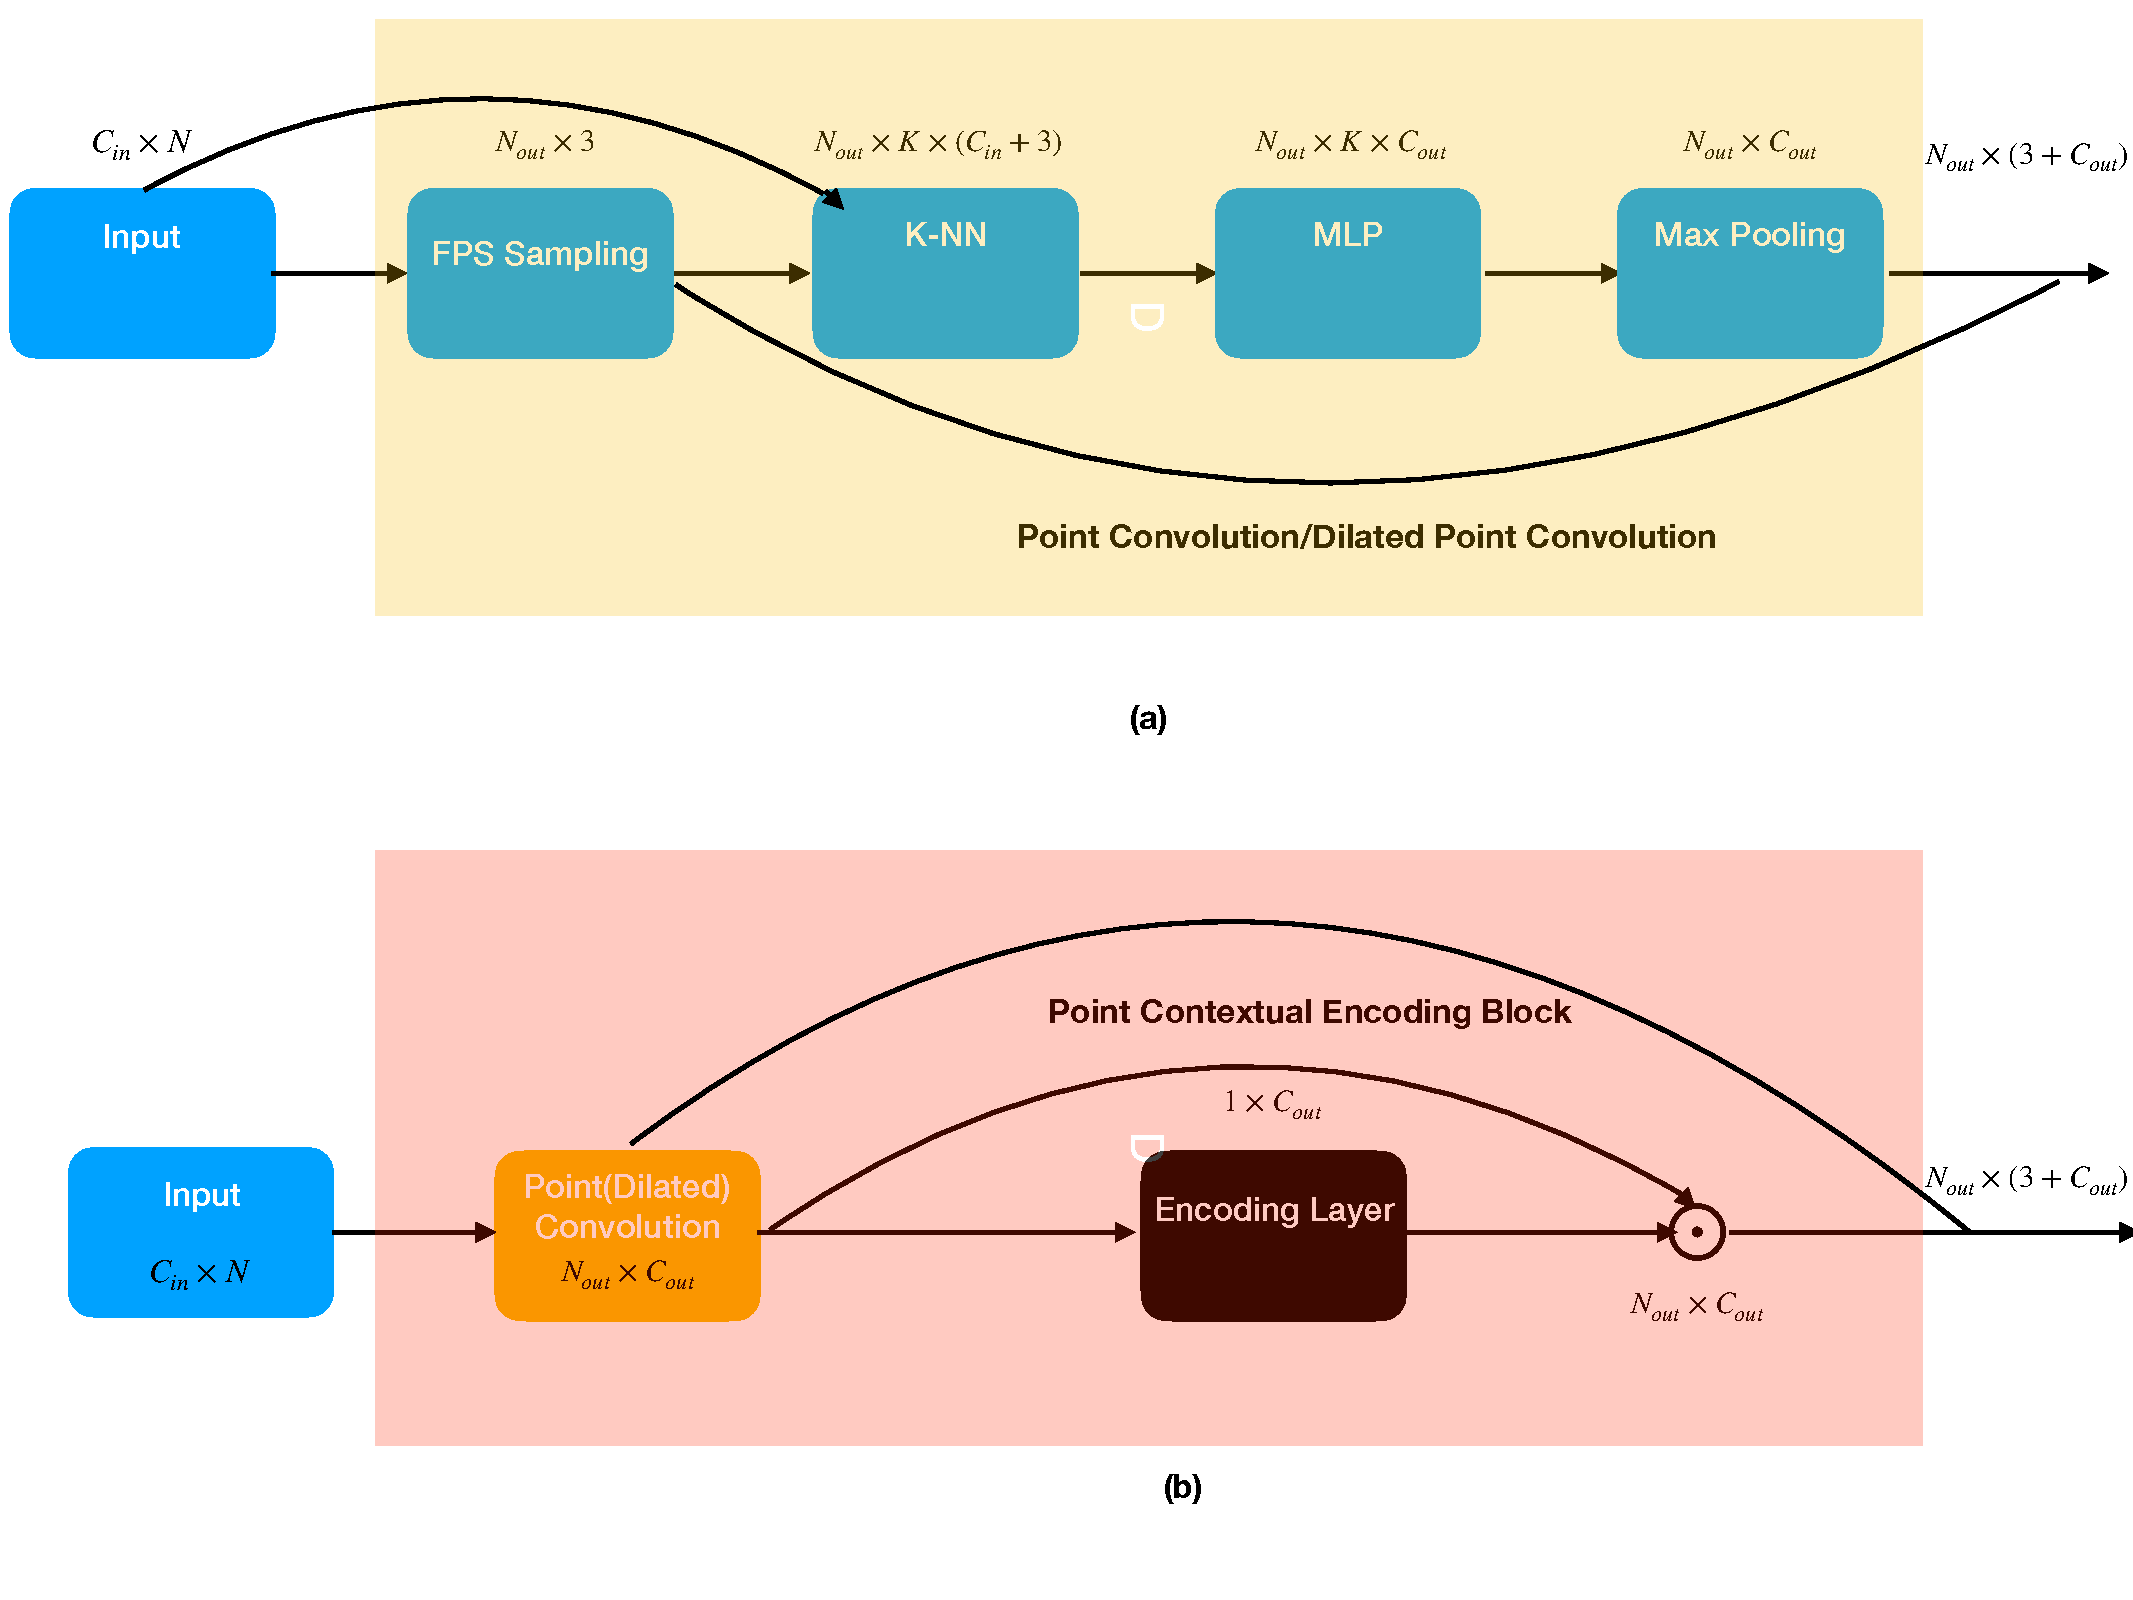
\includegraphics[width=1.0\linewidth]{eccv2020kit/Figure/SA_layer.pdf}
			\end{minipage}
    \caption{The comparison of Point Convolution (a) and Point Contextual Encoding Block(b)}
    \label{fig:PointConv}
\end{figure}

\section{Interpretation of PointNet++ with Point Convolution}

The PointNet++ \cite{pointnet++} consists of a series of SA( Set Abstraction) layers to extract the features. The procedure of the SA layer is illustrated in Figure \ref{fig:PointConv} (a): with the given point set and the feature, it uses the Farthest Point Sampling (FPS) strategy to sub-sample the output points from the input. %and determine the output points. 
Then for each of  the sampled point, the K-NN method is applied to choose the features from the K nearest points. Then the new feature will be computed by passing the information of k points  to a MLP (Multi-Layer Perception) network, a max pooling operator is then appended to reduce the size and then finally concatenate the feature with the coordinates of the output points.

This process can be also formulated by Point Convolution in the followings:

\noindent \textbf{Point Convolution} 
For the point sets, the feature map $X$ is yield by  
\begin{equation} 
X= (f*g)(x)= \sum_{x_{i}\in N_{x}} g(x_{i}-x)f_{i} \label{equation:PointConv}
\end{equation}
where we dub $x_{i}$ as coordinate of the point and $f_{i}$ as its corresponding input feature ,  $g$ is kernel of the convolution.  $N_{x} = \left\{  \left\|x_{i}-x  \right\| \leq r \right\}$ is the set of the points chosen by neighbourhood within certain radius $r$.

In practice, the points of $N_{x}$ are sampled by $k$ nearest neighbours (kNN). And the the kernel $g(x)$ is the Multi-Layer Perception network, denoted by $g(x)=MLP(x)$. This procedure is depicted on Figure \ref{fig:PointConv} (a). and Equation \ref{Equa:PointConv} and \ref{Equa:MLP}.

And the $\theta$ is the hyper parameter of MLP layer. 

\begin{equation}
    X = (f*g)(x) = \sum_{i=1}^{i=k}g(x_{i}-x)f_(x_{i})
    \label{Equa:PointConv}
\end{equation}

\begin{equation}
    g(x) = MLP_{\theta}(x)
    \label{Equa:MLP}
\end{equation}

The dilated point convolution \cite{DPC} choose the k samples by the $d,2d...kdth$ nearest point. And the formula can be written by 
\begin{equation}
    X = (f*g)_{d}(x) = \sum_{i=1}^{i=k}g(x_{id}-x)f_(x_{id})
    \label{Equa:DilatedPointConv}
\end{equation}

\subsection{FP decoding layers}

To recover the feature size back to the original size, the PointNet++ \cite{pointnet++}. 

\begin{equation}
    f^{(i)}(x)=\frac{\sum_{i=1}^{k} w_{i}(x) f_{i}^{j}}{\sum_{i=1}^{k} w_{i}(x)} 
\end{equation}

\begin{equation}
 w_{i}(x)=\frac{1}{d(x,x_{i})^p}
\end{equation}


The k=3,




\section{Method}

%\subsection{The importance of Global Context}
%\label{sec:bayesian}
%The statistics of the  point cloud in the  high-dimensional feature space can be exploited for better  feature representations. We assume this  distribution  on individual point $x$ of the scene $\Omega$ can be represented by $P(x,\Omega)$. 

%However, this idealistic distribution is difficult to estimate . In practice,  the conditional statistics or Probability $P(x|\Omega)$  of the scene $\Omega$ is used  for estimating the  distribution.  The softmax normalization operator widely used in deep neural networks to obtain probability logit for criterion can be regarded an example of  $P(x|\Omega)$.

%According to the  Equation \ref{equation:bayesian}, to approximate the value of $P(x,\Omega)$, the statistics of the scene $P(\Omega)$ should be taken into consideration and this is referred to as the global context.
%\begin{equation}
 %  P(x,\Omega) = P(x|\Omega)\times P(\Omega)
%   \label{equation:bayesian}
%\end{equation}

%The global context $P(\Omega)$ should be multiplied with the conditional distribution $P(x|\Omega)$ to rectify the bias. 

%This principle %serves as  the guideline for our n introduced in Section \ref{section:method} to
%motivates us to introduce the global context in Section \ref{section:method} and combine with this information via  the $\times$ operation.
%re-calibrate the features by multiplying the feature with the global context.



\subsection{Point Context Encoding Block}

In this part, we introduce the  method  to yield  the global context with Point Contextual Encoding layer. %As mentioned in section \ref{sec:bayesian}, 
And this layer will be applied to  
the Point Convolution operator and the global context will be fused  with the original feature of the Point Convolution by multiplying with the global context. Which is similar to \cite{SENet}.  As a result, the point features will be empowered by the global context and this will lead to better performance. 

As shown in Figure \ref{fig:PointConv} (b), this is dubbed as the Point Context Encoding block, and this constitutes the backbone in our design. 

\label{section:method}

\noindent \textbf{Point Contextual Encoding Layer}

% The contextual information of the point sets is crucial for the task of 3D object detection. 
To capture the global contextual feature of the point sets. We leverage the encoding layer in \cite{DeepTEN} to exploit the statistics of the point sets. The encoding layer learns the codebook spontaneously and then encode the features according to  the  residual between the feature and the code words. The global contextual prior will be then be multiplied for re-calibrating the featuremap.

For the feature $X \in \mathbb{R}^{ C \times N}$ $X=\left\{ X_{1} ... X_{N}\right\}$  of the point sets, where $N$ is the number of the point sets and $C$ is the channel number.Let 
the code book $D=\left\{d_{1},d_{2},...d_{K} \right\}$ has $K$ code words to be learned by the network.

The residual  $r_{ik}= x_{i}-d_{k}$ will be weighted summed by $e_{k}=\sum_{i=1}^{N} e_{ik}$
\begin{equation}
e_{ik} = \frac{e^{-s_{k}\left\| r_{ik}\right\|^{2}}}{\sum_{j=1}^{K} e^{-s_{k}\left\| r_{ik}\right\|^{2}} } r_{ik}
\label{encoding}
\end{equation}

The scaling factor $s$ is a learn-able parameter in the process.
To obtain the global context of the scene, the information of the encoders will be aggregated by the sum operation after passing each  of the encoders individually with Batch Normalization \cite{BN} and ReLU operations,denoted with $\phi$,  which is given by
\begin{equation}
    e=\sum_{i=1}^{K} \phi (e_{k})
 \label{aggregation}  
\end{equation}

The computation complexity of the whole procedure is $O(N \times K)$ , which is computation economical.

It should also be noted that when $K=0$, the encoding layer is degenerated into global average pooling introduced in PSPNet \cite{PSPNet}.

To make use of the aggregated information $e$, it  will pass through a fully connected layer and sigmoid activation function and be utilized as  channel-wise attention, which is similar to \cite{SENet}.  This process is given by $\gamma=\sigma(We)$, where the $\sigma$ denotes for the sigmoid activation, and $W$ stands for the weight of the FC (Fully Connected) layer.

The global descriptor $\gamma$ will be multiplied with the input feature $X$ with the channel wise multiplication: $Y=X\odot \gamma$ for it acts as modulator  of the featuremap: For instance, % it will de-emphasize the probability that the furniture appears in the bathroom. And will increase the likely-hood that the pillow that appears on the bed according to the global context obtained from the encoding layer. 
\label{sec:PointEnc}


\subsection{Enc-PointNet++}
The structure of our model is homogeneous with PointNet++ \cite{pointnet++}. It followed the encoder-decoder design which pass through a series of Point Contextual Encoding Blocks in section \ref{sec:PointEnc}, then in the decoder phase, the feature will be up-sampled , fused and  recovered back to its original size. 

\begin{figure}[t]
\begin{minipage}{1.0\textwidth}
    \centering
    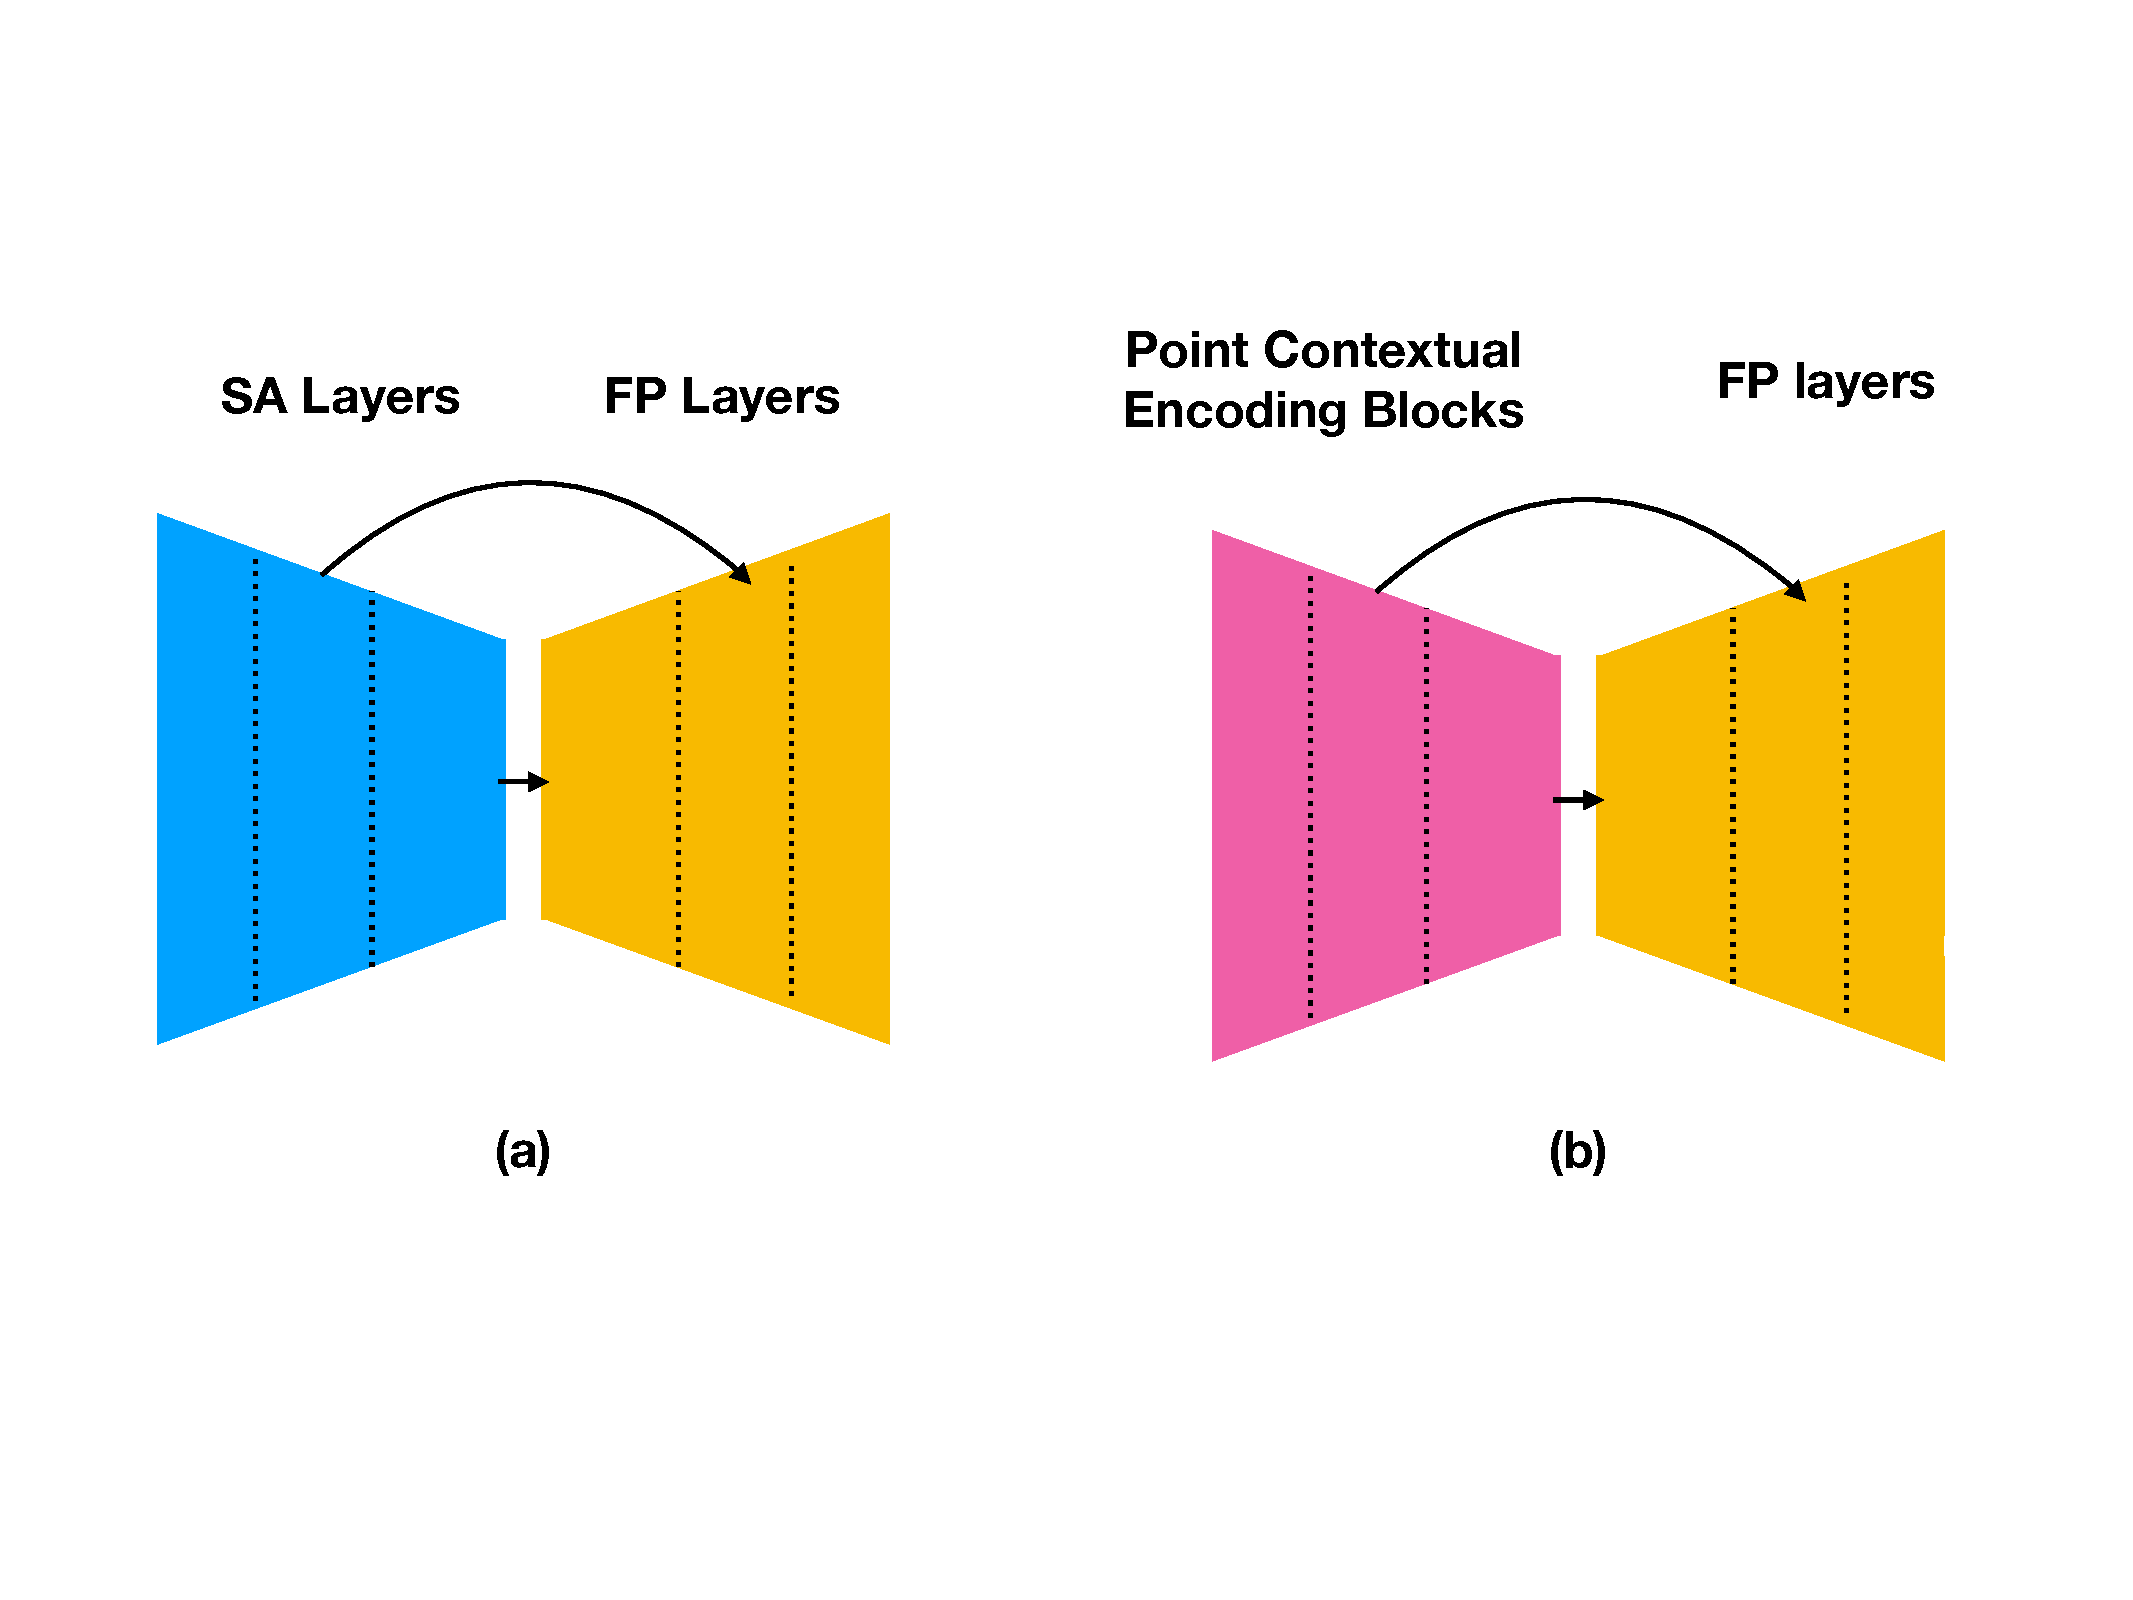
\includegraphics[width=.8\linewidth]{eccv2020kit/Figure/enc_pointnet++.pdf}
    \caption{The structure of PointNet++ in (a) and our Enc-PointNet++ in (b) }
\end{minipage}
\label{fig:enc_pointnet}
\end{figure}

In contrast with the original PointNet++,  the feature from each layer of  Point Convolution will be modulated by the global context.  As a result, the representation ability of  our Enc-PointNet++ module is better than the original PointNet++. %of the SA layers will be enhanced by the global context within its range of scale.  Therefore, the Enc-PointNet++ should be more powerful than its counterpart of PointNet++.

\begin{figure}[t]
\begin{minipage}{1.\textwidth}
    \centering
    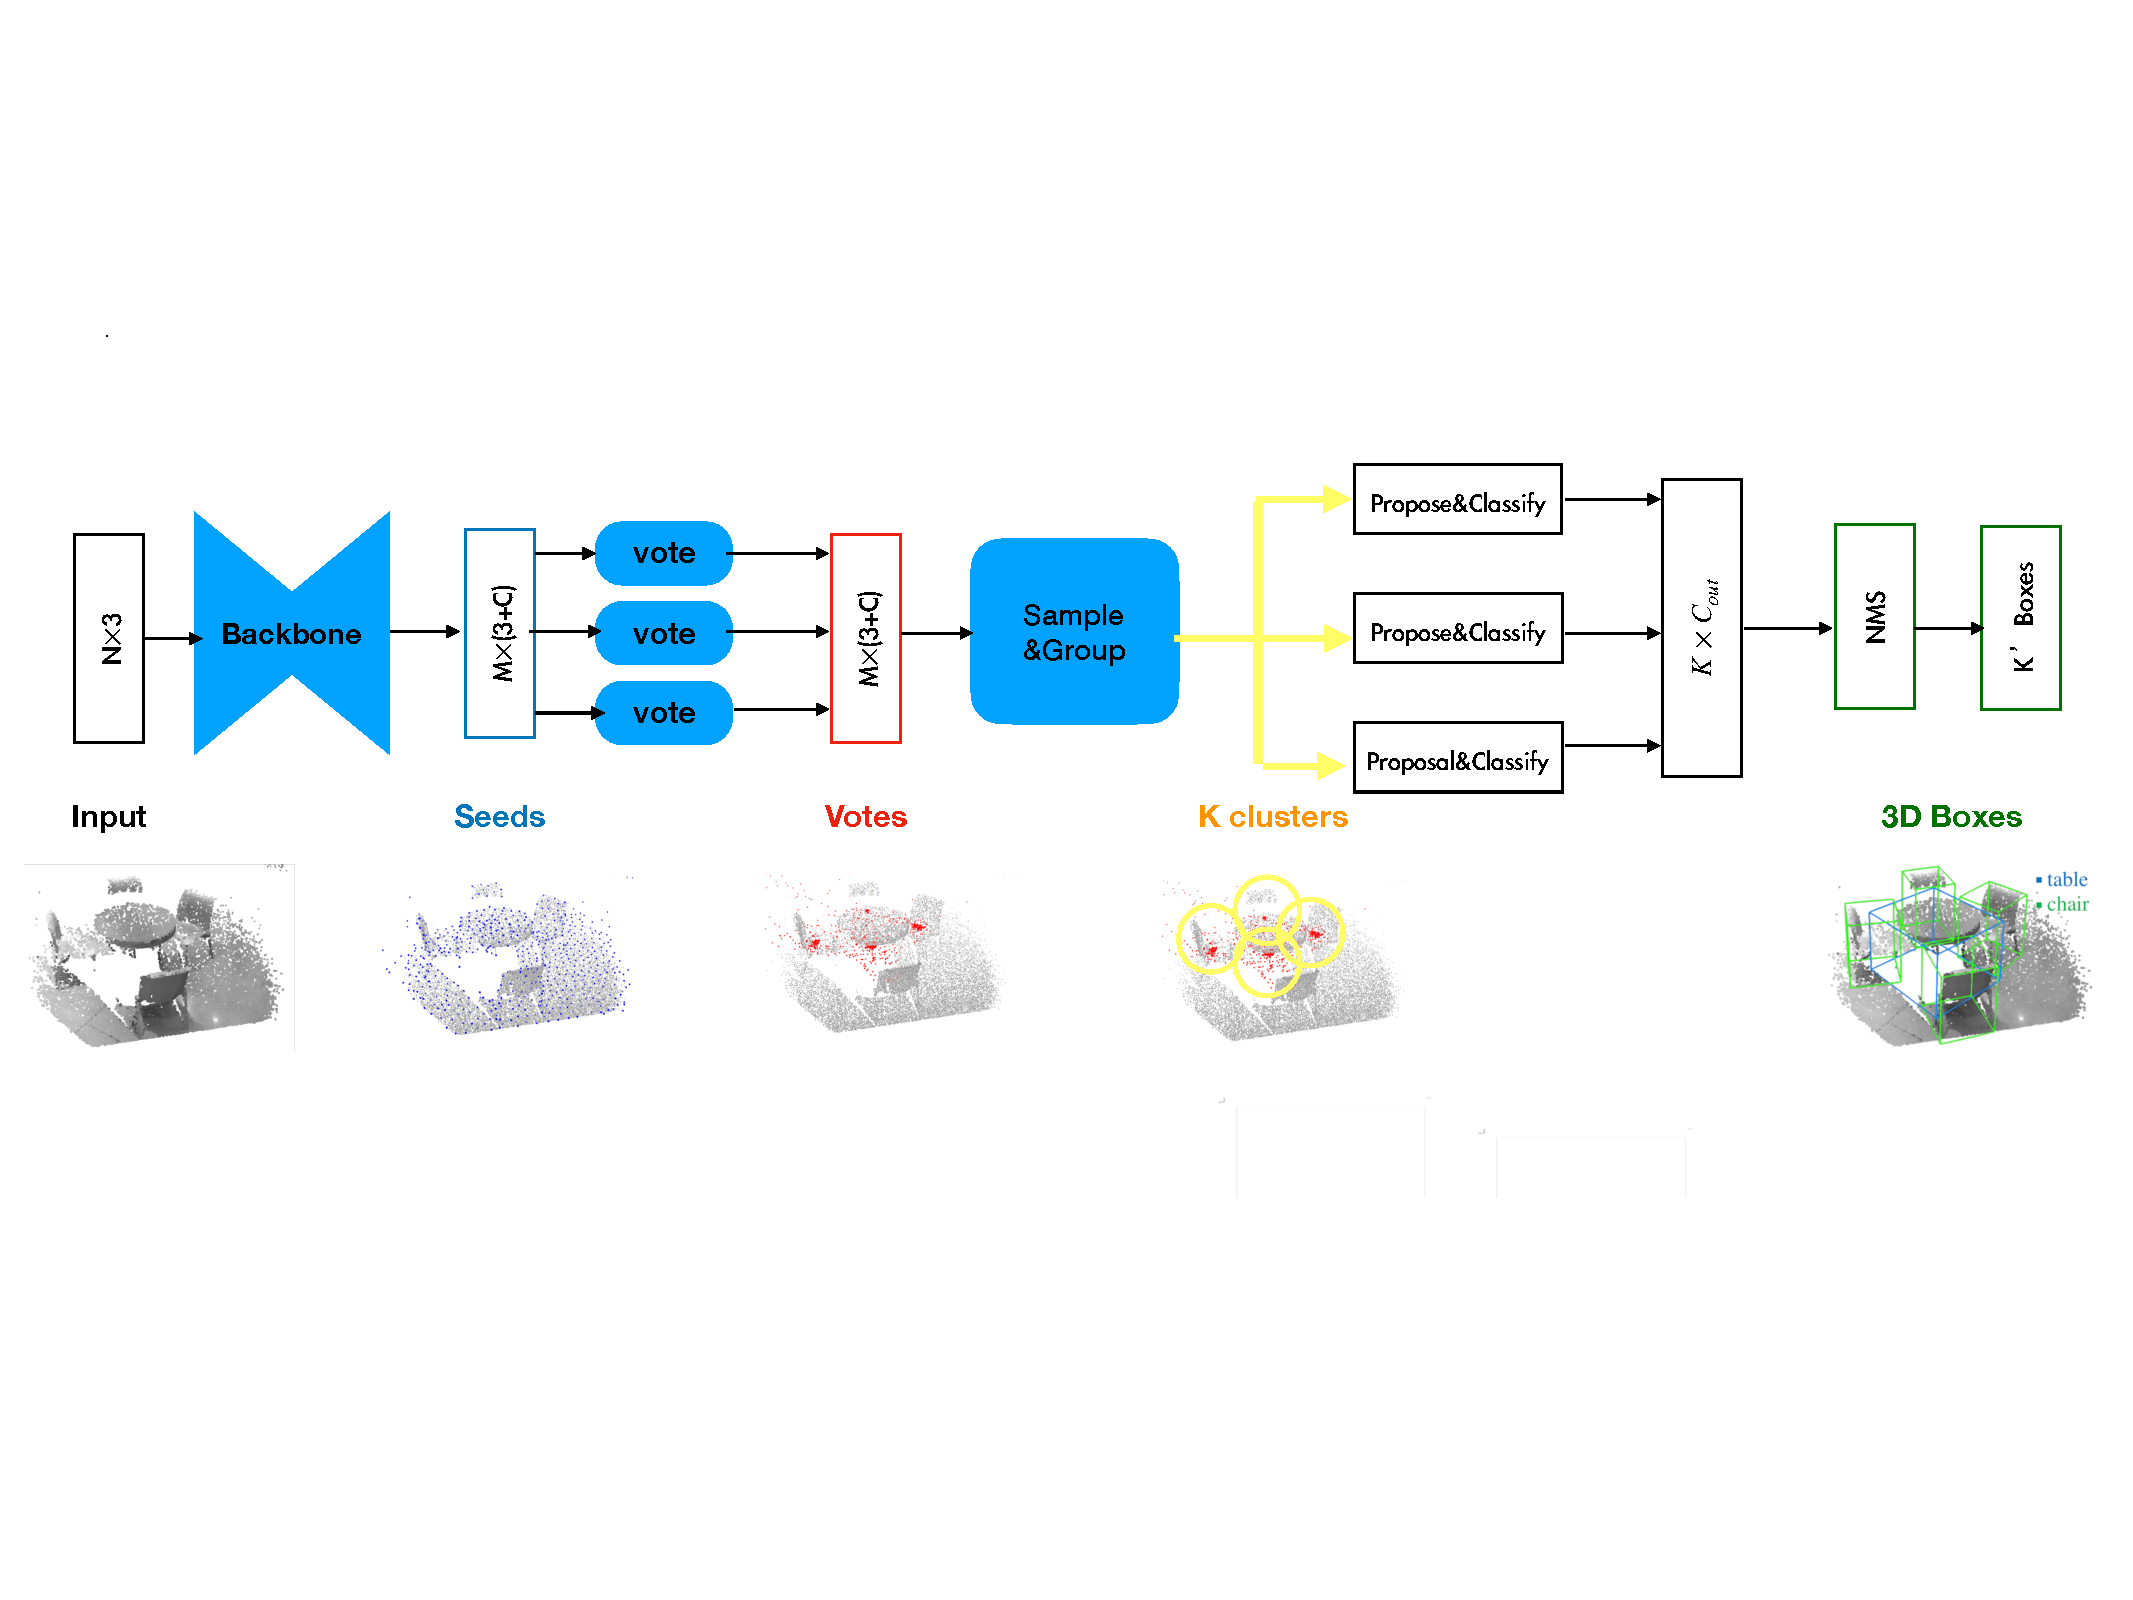
\includegraphics[width=1.0\linewidth]{eccv2020kit/Figure/VoteNet.pdf}
    \caption{The framework of VoteNet \cite{VoteNet}, the M point seeds and the features from the Backbone will be fed into the Voting Layer to choose K clusters, then the proposal layer is appended to predict  bounding boxes and classify the object category. }
\end{minipage}
\label{fig:votenet}
\end{figure}


To verify the efficacy of the Enc-Point++, this backbone will be plugged on the VoteNet \cite{VoteNet}. The procedure of Votenet is depicted in Figure \ref{fig:enc_pointnet}. The features of the point set will be extracted by the Backbone Network. The points in the seeding layer will then be clustered and grouped into 3D boxes. The boxes  will be further refined by the post-processing NMS method.

\section{Experiments}
\label{section:experiment}
In this section, we first conduct a series of ablation studies to verify the efficacy of our module. 

\subsection{Dataset}
SUN RGB-D \cite{SUN_RGBD} for 3D indoor scene understanding consists of around 10k RGB-D images annotated with 64,595 oriented 3D bounding boxes for nearly 40 object categories. In our experiment, following \cite{VoteNet} we split the training/testing set and report 3D detection performance on the 10 most common categories. 

ScanNet \cite{SCannet} provides a wider range of indoor scenes with more densely scanned objects compared with the SUN RGB-D dataset. We use the  1205 scans for training  and 312 scans  for  testing, respectively.  Vertices from meshes  are sampled as the input point clouds. Following the ground-truth annotation mentioned in \cite{VoteNet}, we predict axis-aligned 3D bounding boxes in these scenarios.

In experiments, we follow the same protocol in \cite{VoteNet} and use the metrics, mean average precision (mAP), at IoU threshold 0.25 for evaluation.

\subsection{Implementation Details} 
\noindent\textbf{Architecture}
We  follow the framework of  VoteNet \cite{VoteNet}, as shown in Figure \ref{fig:votenet}, which can be  divided into three   backbone, voting and clustering module, and proposal module.

As for the backbone, the   hyper-parameters and configuration of the PointNet++ backbone is the same with our Enc-PointNet++ for fair comparison. For example, the 1st layer of Point Contextual Encoding block will sample  2048 points from the scene, which is the same with SA1 layer in VoteNet \cite{VoteNet}.

As for the configuration of code word number K, it is the same for each of the Point Contextual Encoding layer for simplicity, we choose $K=32$ for our design, the rationales for this choice will be given in Section \ref{section:}.
 

\noindent\textbf{Training and Inference}
 We adopt the same data augmentation methods with VoteNet \cite{VoteNet} .  Here we also adopted the same optimizer, Adam Optimizer \cite{adam}, which  is utilized with an initial learning rate 0.001. Learning rate is scheduled to be decayed by the factor of 0.1 after 80 epochs and another 0.1 after 120 epochs. There are 180 epochs in total, which is the same with VoteNet\cite{VoteNet}. The whole model is trained on a single Nvidia Titan-X GPU.
 
During inference,  the points of the entire scene are taken as the input. With a \emph{single shot pass}, the region proposals are generated by the framework and further post-processed by 3D NMS method.

\subsection{Ablation Studies}
We set a  series of ablation studies and investigate the relationship of performance with the code word number K, and the comparison of Enc-Point++ and PointNet++,  and the peformance with different layers, which is shown in the Table \ref{tab:codeword}, \ref{tab:ablation_studies}. %between the including the relation ship with 


To show the difference with the PointNet++, for instance, the item \emph{SA2'} means the featuremap of the 2nd layer of  Point Contextual Encoding Blocks in Figure \ref{fig:enc_pointnet}(b), so is SA3', SA4'
The FP operators are kept the same with PointNet++ in VoteNet\cite{VoteNet}, like FP1 and FP2. Though the FP layers are unchanged, 

\noindent{\textbf{Code word number: K}}

To verify the choice of codeword number K in the dictionary, we conducted experiment on SA2' with a series  of numbers K=0,16,32 and the results are shown in Table \ref{tab:codeword}.       

The result shows that the the improvement of global average pooling (K=0) is limited, only 0.5 mAP improvement on ScanNetV2 compared with the baseline SA2 , The  global average pooing widely used for 2D tasks is not effective for the 3D point cloud. It is easy to interpret: unlike 2D image, the distribution of 3D point cloud  is irregular, thus the simple operator of global average pooling is unable to give a true description of the global scene, therefore,  it does not work well for the irregular 3D point clouds.


In theory,  the performance will increase with the code number $K$ because the  complex scenes can be encoded by more independent code words . In practice, we find the performance get saturated when $K=32$. Therefore, we choose the $K=32$ for the following experiments.

\setlength{\tabcolsep}{4pt}
\begin{table*}
\centering
\scalebox{1.0}
{
\begin{tabular}{cccc}
				\toprule
				\multicolumn{2}{c}{\multirow{3}*{Method}} & \multicolumn{2}{c}{mAP@0.25} \\ %\multicolumn{2}{c}{\multirow{3}*{)}}\\
				\cmidrule(lr){3-4}
				%\multicolumn{2}{c}{} & \multicolumn{2}{c}{640$\times$360} & \multicolumn{2}{c}{1280$\times$720} & \multicolumn{2}{c}{1920$\times$1080} & \\
				\multicolumn{2}{c}{} & SUN RGB-D V1 &  ScanNetV2 &\multicolumn{2}{c}{} \\
				%\noalign{\smallskip}
				%\midrule
				\midrule
				\multicolumn{2}{l}{SA2} & 51.2  &51.2   \\
				\multicolumn{2}{l}{SA2'(K=0)} & 51.9 &51.7 \\
				\multicolumn{2}{l}{SA2'(K=16)} & 54.7  &53.1 \\
				\multicolumn{2}{l}{SA2'(K=32)} & 55.0  &53.4 \\	
            \bottomrule	
\end{tabular}
    \caption{Ablation studies of code word K.}
    \label{tab:codeword}}
\end{table*}
%\noindent{\textbf{Large Receptive Field Matters}}
% more stages of dilation helps
\noindent{ \textbf{Comparison with PointNet++}}

Table \ref{tab:ablation_studies} shows the performance of VoteNet \cite{VoteNet} with features from different layers of PointNet++ and Enc-PointNet++. The  detection result has shown that with the same seed layer,  the  performance of Enc-PointNet++   is better than PointNet++. For example the performance of SA3' is 57.2 mAP on SUN-RGBD V1 dataset, better than its counterpart SA3, which is  56.3 mAP.


\setlength{\tabcolsep}{4pt}
\begin{table*}
\centering
\scalebox{1.0}
{
\begin{tabular}{cccc}
				\toprule
				\multicolumn{2}{c}{\multirow{3}*{Method}} & \multicolumn{2}{c}{mAP@0.25} \\ %\multicolumn{2}{c}{\multirow{3}*{)}}\\
				\cmidrule(lr){3-4}
				%\multicolumn{2}{c}{} & \multicolumn{2}{c}{640$\times$360} & \multicolumn{2}{c}{1280$\times$720} & \multicolumn{2}{c}{1920$\times$1080} & \\
				\multicolumn{2}{c}{} & SUN RGB-D V1 &  ScanNetV2 &\multicolumn{2}{c}{} \\
				%\noalign{\smallskip}
				%\midrule
				\midrule
				\multicolumn{2}{l}{FP'} & 58.7  &57.6  \\
				\multicolumn{2}{l}{FP'')} & 57.5 &56.6 \\
            \bottomrule	
\end{tabular}}
    \caption{Ablation studies on decoder.}
    \label{tab:codeword}
\end{table*}

 
\noindent{ \textbf{The use of FP decoder}}

To verify if the encoding layer is still valid for the FP operators, we also  deployed the Point Contextual Encoding layer on FP1 layer, the encoded context feature will be multiplied with the FP1 feature. which is similar to the Point Contextual Encoding Block. We call this feature FP''

The table shows that the encoding layer deployed on FP operator is superfluous, the performance has dropped by 1.0 mAP on both of the benchmarks. Which implies that it is unnecessary to introduce the encoding layer in the decoding phase. 


It has also been pointed  out by \cite{VoteNet} that FP layers in PointNet++ does not necessarily improve the performance , for example the performance of VoteNet with FP3 layer is 57.1 mAP on SUN-RGBD dataset, which is less than the performance of FP2. And also, the performance of FP1 layer is approximately the same with SA3 layer shown in Table \ref{tab:ablation_studies}.

Our result also shows this problem. For instance, the performance of FP2' is 57.9 , which is less than FP1' of 58.7 on the benchmark of ScanNet.

The result shows that the FP decoders is not suitable for the task of object detection. The reason is because the FP operator is a coarse upsampling operator. Therefore, The reason why the performance of ``FP2'' is better may be that the point distribution in ScanNet is not as challenging as SUN-RGBD for the FP decoder.

But our point contextual module still proves to be valid for the challenging object detection methods in spite of the constraint of FP layers.



\setlength{\tabcolsep}{4pt}
\begin{table*}
\centering
\scalebox{1.0}
{
\begin{tabular}{ccccc}
				\toprule
				\multicolumn{2}{c}{\multirow{3}*{Seed Layer Feature}} & \multicolumn{3}{c}{mAP@0.25} \\
				\cmidrule(lr){3-5}
				%\multicolumn{2}{c}{} & \multicolumn{2}{c}{640$\times$360} & \multicolumn{2}{c}{1280$\times$720} & \multicolumn{2}{c}{1920$\times$1080} & \\
				\multicolumn{2}{c}{} & SUN RGB-D V1 & ScanNetV2  \\
				\noalign{\smallskip}
				%\midrule
				\midrule
				\multicolumn{2}{l}{SA2} & 51.2 &51.2 \\

				%\multicolumn{2}{l}{SA2+Point Diffusion(3,6)} & 58.0 &59.5 & 56.9  & \multicolumn{2}{c}{0.94}\\
				%\multicolumn{2}{l}{SA2+Point Diffusion(3,6,12)} &57.9 & 59.6&  59.0 & \multicolumn{2}{c}{1.26}\\
				\midrule
				\multicolumn{2}{l}{SA3} & 56.3 & 54.4 \\
				\multicolumn{2}{l}{SA4} & 55.1 &  47.4   \\
				\multicolumn{2}{l}{ FP1} & 56.6 &  56.6\\
				\multicolumn{2}{l}{ FP2} & 57.7 &  58.6\\
				\midrule
				\multicolumn{2}{l}{SA2'} & 55.0  & 53.4\\
				\multicolumn{2}{l}{SA3'} & 57.2 & 55.4\\
				\multicolumn{2}{l}{ SA4'} & 56.1 & 52.4 \\
				\multicolumn{2}{l}{ FP1'} & \textbf{58.7}& 57.6& \\
				\multicolumn{2}{l}{ FP2'} & 57.9 & \textbf{59.4}& \\
				
				\bottomrule		%\vspace{0.1em}
			\end{tabular}
			}

    \caption{Ablation studies }
    \label{tab:ablation_studies}
\end{table*}


\setlength{\tabcolsep}{4pt}
\begin{table*}
		\begin{center}
			\scalebox{0.75}{
			\begin{tabular}{l|c|cccccccccc|c}
				\toprule
				Method & Input & \rotatebox{90}{bathtub}&\rotatebox{90}{bed}& \rotatebox{90}{book self}& \rotatebox{90}{chair} &\rotatebox{90}{desk}&\rotatebox{90}{dresser}& \rotatebox{90}{nightstand}&\rotatebox{90}{sofa}&\rotatebox{90}{table}&\rotatebox{90}{toilet}&mAP \\
				\noalign{\smallskip}
				\midrule
				\noalign{\smallskip}
				F-PointNet \cite{FrustumPointNet}&Geo+RGB&43.3&81.1&\textbf{33.3}&64.2&24.7&32.0&58.1&61.1&\textbf{51.1}&\textbf{90.9} &54.0 \\
				VoteNet \cite{VoteNet}&Geo Only&74.4&83.0&28.8&\textbf{75.3}&22.0&29.8&62.2&64.0&47.3&90.1 &57.7 \\
				\textbf{Ours}&Geo Only&\textbf{76.4} & \textbf{ 84.15} & 28.9 &72.9& \textbf{25.5} &\textbf{33.1}  &\textbf{63.9} & \textbf{65.6} &49.2 &87.2& \textbf{58.7}\\	

							%&  &  & &  \\
				 %& Res18 & 8.3G & 42.7M & 61.58\\
				\bottomrule
			\end{tabular}}
		\end{center}
		\caption{Comparison with the state of the art algorithm on SUN RGB-D V1 benchmark.}
		\label{tab:SUNRGBD_v1}
\end{table*}


\setlength{\tabcolsep}{4pt}
\begin{table*}
\begin{center}
\scalebox{0.53}{
\begin{tabular}{l|cccccccccccccccccc|c}
\toprule
& \rotatebox{90}{cab} &\rotatebox{90}{bed}&\rotatebox{90}{chair}&\rotatebox{90}{sofa}&\rotatebox{90}{table}&\rotatebox{90}{door}&\rotatebox{90}{wind}&\rotatebox{90}{bkshf}&\rotatebox{90}{pic}&\rotatebox{90}{cntr}&\rotatebox{90}{desk}&\rotatebox{90}{curt}&\rotatebox{90}{fridg}&\rotatebox{90}{showr}&\rotatebox{90}{toil}&\rotatebox{90}{sink}&\rotatebox{90}{bath}&\rotatebox{90}{ofurn}&mAP \\
\noalign{\smallskip}
\midrule
\noalign{\smallskip}
3DSIS Geo \cite{3d-sis}& 12.75&63.14&65.98&46.33&26.91&7.95&2.79&2.3&0.00&6.92&33.34&2.47&10.42&12.17&74.51&22.87&58.66&7.05&25.36\\
VoteNet \cite{VoteNet}&36.27&\textbf{87.92}&\textbf{88.71}&\textbf{89.62}&58.77&\textbf{47.32}&\textbf{38.10}&44.62&\textbf{7.83}&56.13&\textbf{71.69}&\textbf{47.23}&45.37&57.13&\textbf{94.94}&54.70&\textbf{92.11}&37.20&58.65\\
\midrule
\textbf{Ours}&\textbf{37.64}&87.79 &88.70&89.58&\textbf{60.70}&46.89 &35.89&\textbf{51.40}&2.57&\textbf{60.01}&70.68&43.97& \textbf{48.00}&\textbf{60.64}&94.41&\textbf{59.07}&89.83&\textbf{42.01}&\textbf{59.41}\\

\bottomrule

\end{tabular}}
\end{center}
\caption{Comparison of our method with state of the art algorithm on ScanNetV2, evaluated with mAP @0.25.}
\label{tab:SCanNet0.25}
\end{table*}





\setlength{\tabcolsep}{4pt}
\begin{table*}
\begin{center}
\scalebox{0.54}{
\begin{tabular}{l|cccccccccccccccccc|c}
\toprule
%& cab &bed&chair&sofa&table&door&wind&bkshf&pic&cntr&desk&curt&fridg&showr&toil&sink&bath&ofurn&mAP\\
& \rotatebox{90}{cab} &\rotatebox{90}{bed}&\rotatebox{90}{chair}&\rotatebox{90}{sofa}&\rotatebox{90}{table}&\rotatebox{90}{door}&\rotatebox{90}{wind}&\rotatebox{90}{bkshf}&\rotatebox{90}{pic}&\rotatebox{90}{cntr}&\rotatebox{90}{desk}&\rotatebox{90}{curt}&\rotatebox{90}{fridg}&\rotatebox{90}{showr}&\rotatebox{90}{toil}&\rotatebox{90}{sink}&\rotatebox{90}{bath}&\rotatebox{90}{ofurn}&mAP\\

\noalign{\smallskip}
\midrule
\noalign{\smallskip}
3DSIS Geo \cite{3d-sis}& 5.06&42.19&50.11&31.75&15.12&1.38&0.00&1.44&0.00&0.00&13.66&0.00&2.63&3.00&56.75&8.68&28.52&2.55&14.60\\
VoteNet \cite{VoteNet}&8.07&76.06&67.23&68.82&42.36&15.34&6.43&28.00&\textb{1.25}&9.52&\textbf{37.52}&11.55&27.80&\textbf{9.96}&\textbf{86.53}&16.76&78.87&11.69&33.54\\
\midrule
\textbf{ Ours}&\textbf{8.48}&\textbf{76.16}&\textb{68.77}&\textb{69.28}&\textb{45.20}&\textbf{17.05}&\textbf{11.60}&35.86&0.24&13.17&34.09&\textbf{11.94}&\textbf{30.24}&8.47&83.41&\textb{19.11}&\textb{82.21}&\textbf{14.18}&\textbf{34.99}\\
\bottomrule
\end{tabular}}
\end{center}
\caption{Comparison of our method with state of the art algorithm on ScanNetV2, evaluated with mAP @0.5.}
\label{tab:SCanNet0.5}
\end{table*}


\subsection{Main Results}

The Table \ref{tab:ablation_studies} shows the detailed ablation studies on the bencmark of SUN-RGBD and ScanNet. In this part, we compare our result with the previous state of the art method, including VoteNet and F-PointNet, the result shows that the our methods have outperformed the state-of-the-art.

More details can be found in Table and  Table .



\subsection{Point Cloud Segmentation}
ShapeNet  dataset \cite{}, contains 16,881 shapes from 16 categories, annotated with 50 parts in total. The  categories of the labels are summarized into five parts.  We use mIoU as the metrics for this 

\noindent{\textbf{Implementations:}} The configuration of the Enc-PointNet++ is the same with \href{https://github.com/yanx27/Pointnet_Pointnet2_pytorch/blob/master/models/pointnet2_part_seg_msg.py}{part segmentation} to show the efficacy of the Point Contextual Encoding module. 


The result in Table \ref{}. shows that XXXXXX. The comparison with other methods are  listed in XXXX.


\subsection{Point Cloud Classification}

We also tested the performance of Enc-PointNet++  for the task of point cloud classification. We choose the ModelNet40 benchmark to evaluate our method.

The  ModelNet 40 consists of 12,311 CAD models belonging to 40 catergories. There are 9,843 models and 2,486 models for training and testing splits, respectively. 

\noindent{\textbf{Implementations: }}We make the following adjustments for this task. We replaced the FP layers 3 fully-connected layers . The Batch Normalization \cite{} operator, followed by the dropout layer is applied to the output first two FC layers to reduce the overfitting. The  dropout rates of the first two layers with dropout are 0.4 and 0.5 , respectively. The output of the third FC layer is applied to the softmax loss for classification. For the configuration of the Point Contextual Encoding module, it is identical with the configurations of the  \href{https://github.com/yanx27/Pointnet_Pointnet2_pytorch/blob/master/models/pointnet2_cls_msg.py}{Code} . The normal vector is also taken as the input. The codeword number is also 32 for each of the blocks.

We find that even 
The comparisons with other results can be seen in Table \ref{tab:ModelNet}. We can seen that the performance  even for the simple 

\begin{table}[t]
    \centering
    \begin{tabular}{c|cc}
    \toprule
    Method & mAcc & OA \\
    \midrule
    %\midrule
      PointNet& 86.2 & 89.2\\
      PointNet++& - &91.9\\    
      SpecGCN &-& 92.1\\
      DGCNN &90.2 &92.2\\
      PointCNN &88.1& 92.2\\
      PointWeb &89.4&92.3\\
      \midrule
      PointNet++-MSG-Normal& 89.7& 92.8 \\
      Enc-PointNet++-MSG-Normal& \textbf{89.8} & \textbf{93.0}\\
     \bottomrule
    \end{tabular}
    \caption{The performance  on ModelNet40 benchmark}
    \label{tab:ModelNet}
\end{table}




Configurations





%In this part, we will introduce the performance for the prevailing 3D benchmarks, SUN RGB-D \cite{SUN_RGBD} and ScanNet \cite{SCannet}, respectively. 
%\noindent\textbf{SUN RGB-D} The results on the SUN RDB-D V1 are illustrated in Table \ref{tab:ablation_studies}. The performance of SA2' is 55.0 mAP, as we discussed above. With one stage of our module involved, the SA2' + Dense Point Diffusion V2(3) has reached the performance of 58.7 mAP, which is comparable with the best performance of XXXX V1.

%The performance still continue to increase with an extra stage involved, with SA2' + Dense Point Diffusion V2(3,6) reached performance of \emph{59.2} mAP. Which is 0.5 mAP higher than the previous state of the art XXXXV1. The comparison with other state-of-the-art method is shown in Table \ref{tab:SUNRGBD_v1}.

%Since the scenarios of SUN RGB-D is limited, the receptive field of the module is already big enough when two stages of the module are involved. And more stages does not necessarily  improve the performance, which is similar to the conclusion of XXXV1.  In particular, the performance of SA2' + Dense Point Diffusion V2(3,6,12) is 58.8 mAP, 0.4 mAP less than SA2'+ Dense Point Diffusion V2(3,6).

%We can draw similar conclusions on SUN RGB-D V2, and the peak performance is a \emph{60.9} mAP.



%\noindent\textbf{ScanNet}  
%We deploy our module on a more challenging benchmark of ScanNet, as shown in Table \ref{tab:ablation_studies}. The result shows that the Point Contextual Encoding block is effective even on a more challenging dataset, with SA2' 53.4 mAP on the benchmark and outperforms the SA2 with  2.2 mAP.
%The performance of SA2' + Dense Point Diffusion V2(3) and SA2' + Dense Point Diffusion V2(3,6) on ScanNet are 58.2 mAP and 59.3 mAP respectively.

%In contrast with SUN RGB-D, the performance of our module still increases with the third stage involved. The performance is 59.8 and the details is shown in Table \ref{tab:SCanNet0.25}. Compared with the counterpart of SA2 + Dense Point Diffusion (3,6 ,12) in XXXXV1, the improvement by the module seems to be slight, with only 0.15 mAP increase in the performance. But on a stricter evaluation metrics of mAP @ 0.5 IoU, the performance of SA2' + Dense Point Diffusion V2(3,6,12)  has reached the 38.0 mAP, which is 2.3 mAP higher than SA2 + Dense Point Diffusion (3,6 ,12) in Table \ref{tab:SCanNet0.5} . The comparison with other methods are also listed in Table \ref{tab:SCanNet0.5} that our method has outperformed the VoteNet \cite{VoteNet} with 4.5 mAP. The result has shown it clearly that our method is better suited for challenging scenarios and high performance 3D detection tasks.
\section{Conclusions}

%The paper ends with a conclusion. 


\clearpage\mbox{}Page \thepage\ of the manuscript.
\clearpage\mbox{}Page \thepage\ of the manuscript.

This is the last page of the manuscript.
\par\vfill\par
Now we have reached the maximum size of the ECCV 2020 submission (excluding references).
References should start immediately after the main text, but can continue on p.15 if needed.

\clearpage
% ---- Bibliography ----
%
% BibTeX users should specify bibliography style 'splncs04'.
% References will then be sorted and formatted in the correct style.
%
\bibliographystyle{splncs04}
\bibliography{egbib}
\end{document}
